\documentclass[12pt]{article}
%Published using the GNU General Public License v3.0
\usepackage{graphicx}
\usepackage{hyperref}
\usepackage{array}
\usepackage{ifthen}
%\usepackage{fancyhdr}
\usepackage[latin1]{inputenc}
\usepackage[a4paper,left=2cm, right=0.5cm,top=3cm,landscape]{geometry}
\usepackage{afterpage}
\usepackage{pdfpages}


\title{HAM Logbook}
\author{DB3DE}
\date{\today}

%%%%%%%%%%%%%%%%%%%%%%%%%%%%%%%%%%%%%%%%%%%%%%%%%%%%%%%%%%%
%% Start here editing!
%%%%%%%%%%%%%%%%%%%%%%%%%%%%%%%%%%%%%%%%%%%%%%%%%%%%%%%%%%%

\newcommand{\logpages}{20}      %How many logpages do you want?
\newcommand{\callsign}{DB3DE}   %What is your callsign
\newcommand{\startdate}{}       %What is the startdate of this logbook - put \today for ... today
\newcommand{\lastdate}{}        %Fill this if you want a stopdate 
\newcommand{\includerst}{}      %include the RST mapping at the last pages - remove by commenting using a %
\newcommand{\includebandplan}{} %include the bandplan files - remove by commenting using a %

%%%%%%%%%%%%%%%%%%%%%%%%%%%%%%%%%%%%%%%%%%%%%%%%%%%%%%%%%%%
%% Stop here editing!
%%%%%%%%%%%%%%%%%%%%%%%%%%%%%%%%%%%%%%%%%%%%%%%%%%%%%%%%%%%


%%%%%%%%%%%%%%%%%%%%%%%%%%%%%%%%%%%%%%%%%%%%%%%%%%%%%%%%%%%
%% Header + Footer
%%%%%%%%%%%%%%%%%%%%%%%%%%%%%%%%%%%%%%%%%%%%%%%%%%%%%%%%%%%

\usepackage{fancyhdr}
\setlength{\headheight}{15.2pt}
\pagestyle{fancy}
\pagenumbering{arabic}
\lhead[NA]{\hspace{1cm}{Logbook \callsign}}
\rhead[NA]{\thepage /\logpages }
\cfoot[]{}

%%%%%%%%%%%%%%%%%%%%%%%%%%%%%%%%%%%%%%%%%%%%%%%%%%%%%%%%%%%
%% Leere Seite
%%%%%%%%%%%%%%%%%%%%%%%%%%%%%%%%%%%%%%%%%%%%%%%%%%%%%%%%%%%
\newcommand\blankpage{%
    \null
    \thispagestyle{empty}%
    \addtocounter{page}{-1}%
    \newpage}

%%%%%%%%%%%%%%%%%%%%%%%%%%%%%%%%%%%%%%%%%%%%%%%%%%%%%%%%%%%
%% Log Seite
%%%%%%%%%%%%%%%%%%%%%%%%%%%%%%%%%%%%%%%%%%%%%%%%%%%%%%%%%%%
\newcommand{\logseite}{
  \hoffset=-1.82cm{
%  \hoffset=0cm{
    \begin{tabular}{ r|c@{\hspace{-0cm}}|c@{\hspace{0.8cm}}|c@{\hspace{0.75cm}}|c@{\hspace{0.75cm}}|c@{\hspace{1.0cm}}|c@{\hspace{1.2cm}}|c|c|c|c|c|c@{\hspace{3.6cm}}|l@{\hspace{-0cm}}|l@{\hspace{-0cm}}| }
  
    % 
      \cline{2-15} \cline{2-15}  
      %\textbf{
        & \textbf{QSO} & \textbf{Date} & \textbf{UTC} & \textbf{UTC} & \textbf{station} & \textbf{operator} & \textbf{band} & \textbf{mode} & \textbf{pwr} & \textbf{sig.} & \textbf{sig.} & \textbf{remarks} & \textbf{QSL}  & \textbf{QSL}  \\
        & Nr. &        & in  & out &         &          & \textbf{frequ}    &      &     & in   & out  &         & send & rcvd \\ \cline{2-15}\cline{2-15}
      %}
    
       \small{1}&&&&&&&&&&&&&&\\ &&&&&&&&&&&&&&\\ \cline{2-15}
       \small{2}&&&&&&&&&&&&&&\\ &&&&&&&&&&&&&&\\ \cline{2-15}
       \small{3}&&&&&&&&&&&&&&\\ &&&&&&&&&&&&&&\\ \cline{2-15}
       \small{4}&&&&&&&&&&&&&&\\ &&&&&&&&&&&&&&\\ \cline{2-15}
       \small{5}&&&&&&&&&&&&&&\\ &&&&&&&&&&&&&&\\ \cline{2-15}
       \small{6}&&&&&&&&&&&&&&\\ &&&&&&&&&&&&&&\\ \cline{2-15}
       \small{7}&&&&&&&&&&&&&&\\ &&&&&&&&&&&&&&\\ \cline{2-15}
       \small{8}&&&&&&&&&&&&&&\\ &&&&&&&&&&&&&&\\ \cline{2-15}
       \small{9}&&&&&&&&&&&&&&\\ &&&&&&&&&&&&&&\\ \cline{2-15}
       \small{10}&&&&&&&&&&&&&&\\ &&&&&&&&&&&&&&\\ \cline{2-15}
       \small{11}&&&&&&&&&&&&&&\\ &&&&&&&&&&&&&&\\ \cline{2-15}
       \small{12}&&&&&&&&&&&&&&\\ &&&&&&&&&&&&&&\\ \cline{2-15}
       \small{13}&&&&&&&&&&&&&&\\ &&&&&&&&&&&&&&\\ \cline{2-15}
       \small{14}&&&&&&&&&&&&&&\\ &&&&&&&&&&&&&&\\ \cline{2-15}
     \end{tabular}
  }
}


\begin{document}

%leere Seite nach der Titelseite
\afterpage{\blankpage}

%%%%%%%%%%%%%%%%%%%%%%%%%%%%%%%%%%%%%%%%%%%%%%%%%%%%%%%%%%%
%% Header Page
%%%%%%%%%%%%%%%%%%%%%%%%%%%%%%%%%%%%%%%%%%%%%%%%%%%%%%%%%%%

\begin{titlepage}
   \begin{center}
       \vspace*{0cm}
 
       \textbf{\LARGE{Amateurfunk Logbook}}
 
    
 
       \vspace{1.5cm}
 
       \textbf{\large{\callsign}}
 
       \vfill
 

 
       \vspace{0.8cm}
 
       
\includegraphics[width=0.12\textwidth]{darc_logo}

 
    \vspace{1.5cm}
	\textbf{
%		\hspace{6cm}
		\LARGE{Start date: \startdate}
		\hspace{2cm}\LARGE{Stop date: \lastdate}
 }
        \end{center}  
\end{titlepage}
\newpage


%%%%%%%%%%%%%%%%%%%%%%%%%%%%%%%%%%%%%%%%%%%%%%%%%%%%%%%%%%%
%% Generiere Logbook seiten
%%%%%%%%%%%%%%%%%%%%%%%%%%%%%%%%%%%%%%%%%%%%%%%%%%%%%%%%%%%


\setcounter{page}{1}
\newpage
  \newcounter{ct}

  \setcounter{ct}{1}
  \whiledo{\value{ct} < \logpages}%
  {%
    \logseite\newpage
    \stepcounter{ct}
  }
  \logseite

%%%%%%%%%%%%%%%%%%%%%%%%%%%%%%%%%%%%%%%%%%%%%%%%%%%%%%%%%%%
%% Addons
%%%%%%%%%%%%%%%%%%%%%%%%%%%%%%%%%%%%%%%%%%%%%%%%%%%%%%%%%%%
\ifdefined\includerst

	\lhead[NA]{\hspace{1cm}{Logbook \callsign}}
	\rhead[NA]{\thepage }
	
	\twocolumn
	\LARGE{\textbf{RST System}}\\
	
	\vspace{0.5cm}
	
	
	\LARGE{
	\textbf{R} Verst\"andlichkeit}
	\normalsize{
	
	\begin{tabular}{||c|l||}
	\hline
	Code & Beurteilung\\
	\hline
	 1& 	nicht lesbar\\
	 2& 	zeitweise lesbar\\
	 3& 	mit Schwierigkeiten lesbar\\
	 4& 	ohne Schwierigkeiten lesbar\\
	 5& 	einwandfrei lesbar \\
	 \hline\hline
	\end{tabular}
	\vspace{0.5cm}
	
	\LARGE{
	\textbf{S} Signalst\"arke}
	
	\normalsize{
	\begin{tabular}{||c|l||}
	\hline
	Code & Beurteilung\\
	\hline
	 1& 	nicht lesbar\\
	 2& 	zeitweise lesbar\\
	 3& 	mit Schwierigkeiten lesbar\\
	 4& 	ohne Schwierigkeiten lesbar\\
	 5& 	einwandfrei lesbar \\
	 \hline\hline
	\end{tabular}}\newpage
	
	\LARGE{
	\textbf{T} Tonqualit\"at\
	
	\normalsize{
	\begin{tabular}{||c|l||}
		\hline
		Code & Beurteilung\\
		\hline
		1 & 	\"au\ss{}erst roher Wechselstrom \\
		2 & 	\"au\ss{}erst roher unmusikalischer \\
		  &     Wechselstrom \\
		3 & 	roher Wechselstrom leicht unmusikalisch \\
		4 & 	leicht roher Wechselstrom mittelm\"a\ss{}ig  \\
		  &     musikalisch\\
		5 & 	musikalisch modulierter Ton \\
		6 & 	modulierter Ton leichter Triller \\
		7 & 	unstabiler Ton \\
		8 & 	gefilterter Ton mit z. B.: etwas  \\
		  &     Brummmodulation\\
		9 & 	reiner Ton \\
		 \hline\hline
	\end{tabular}
	}
	}
\fi

\ifdefined\includebandplan
   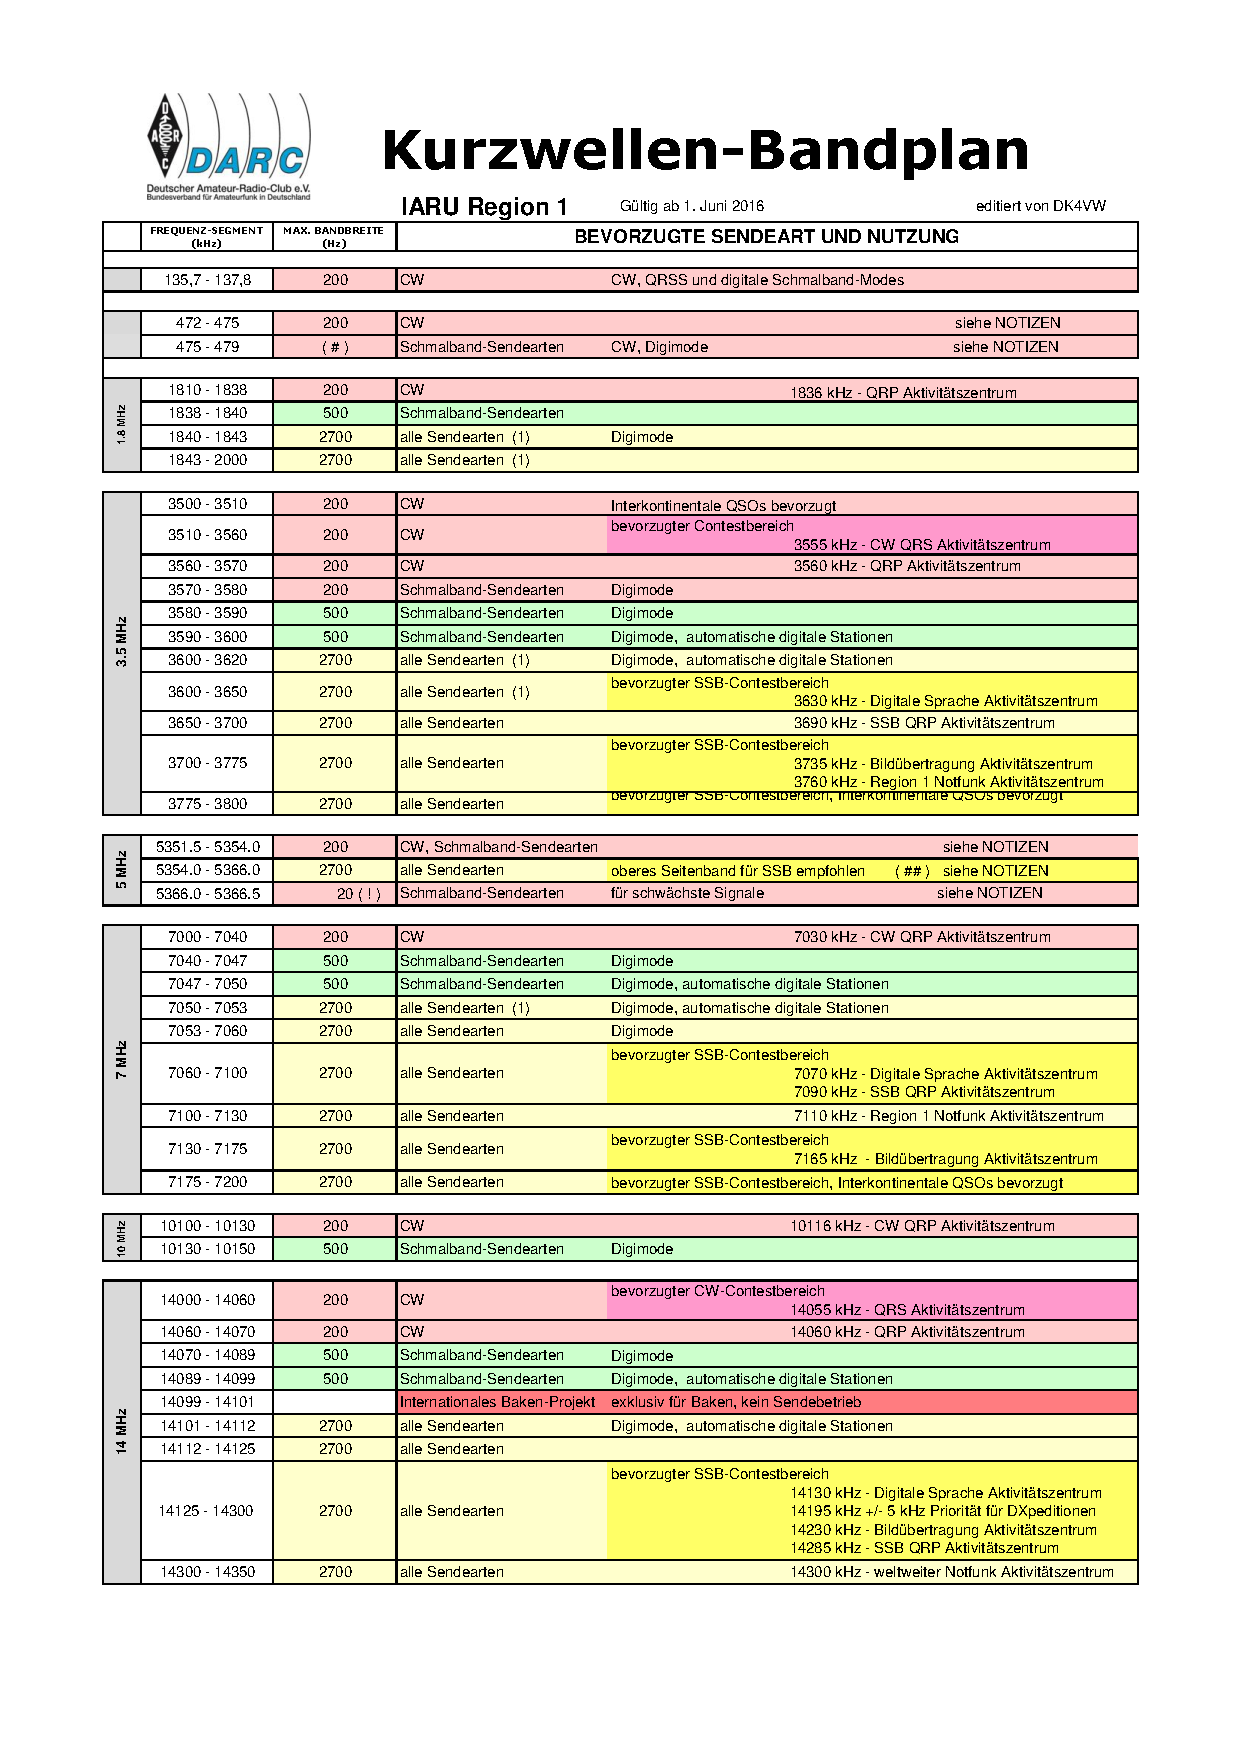
\includepdf[pages=-,nup=2x1,offset=30 -20]{./bandplans/bandplan_KW.pdf}
   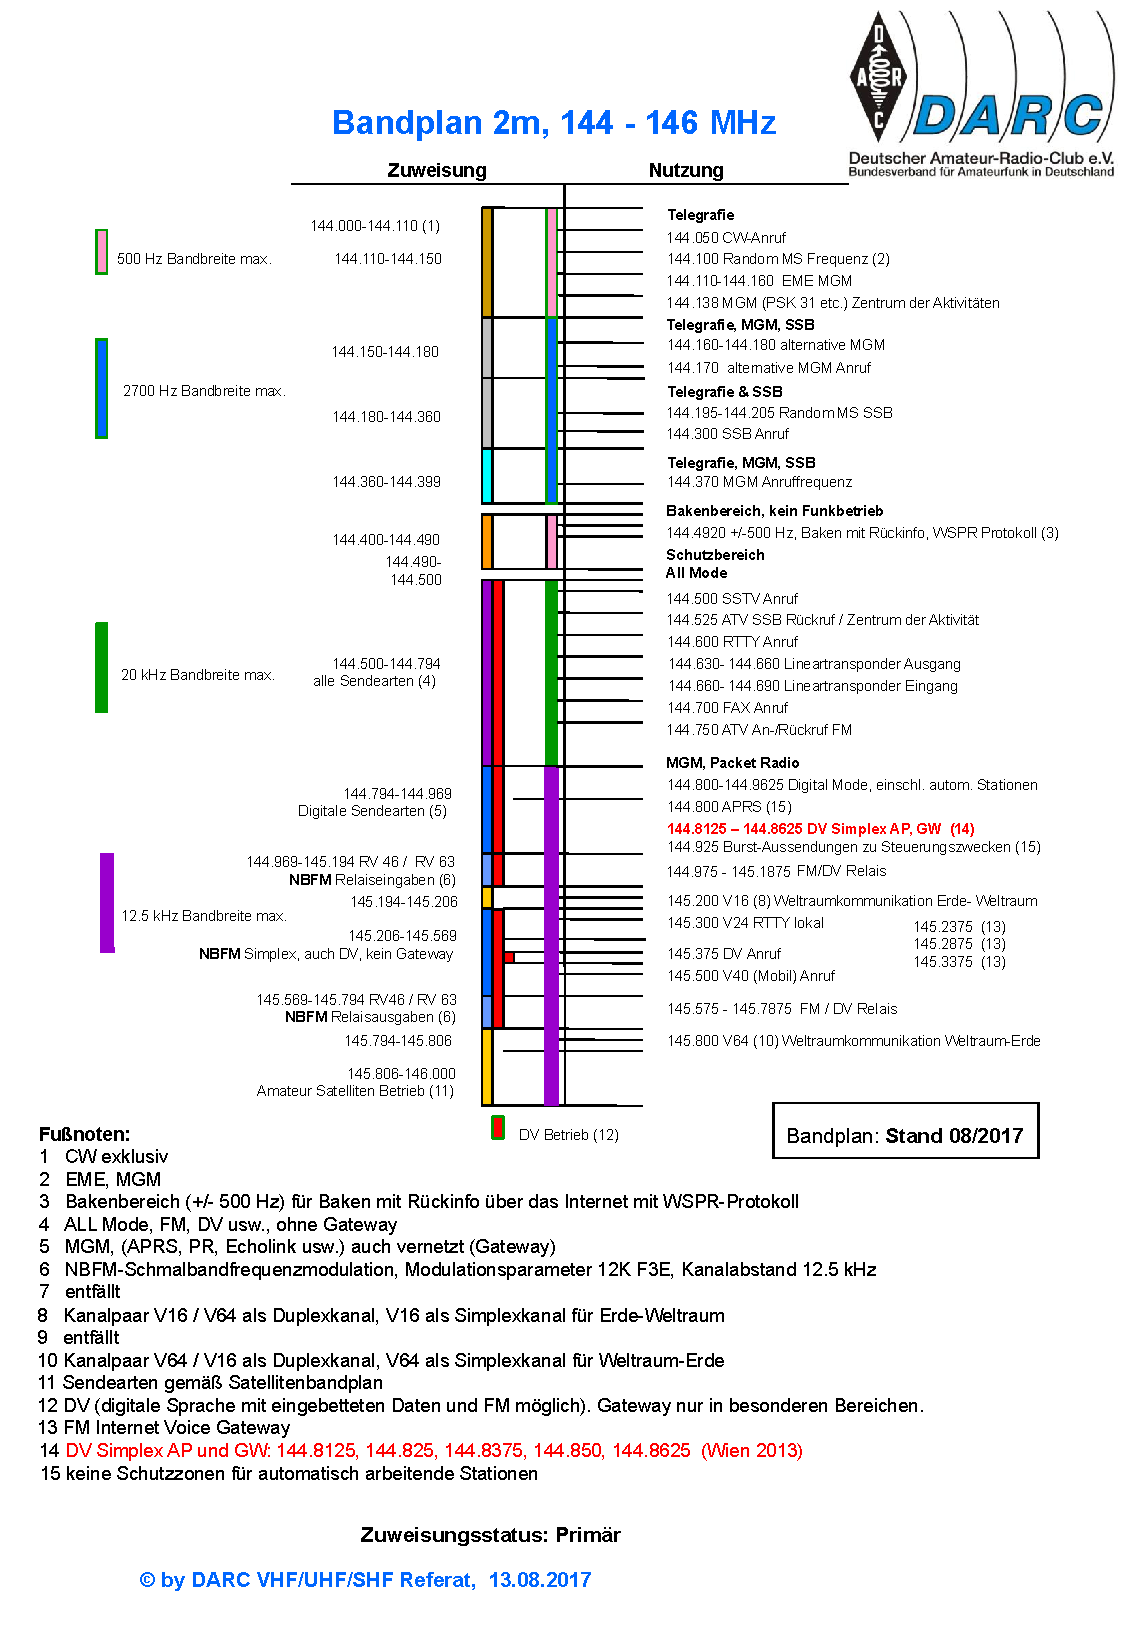
\includepdf[pages=-]{./bandplans/bandplan_2m.pdf}
   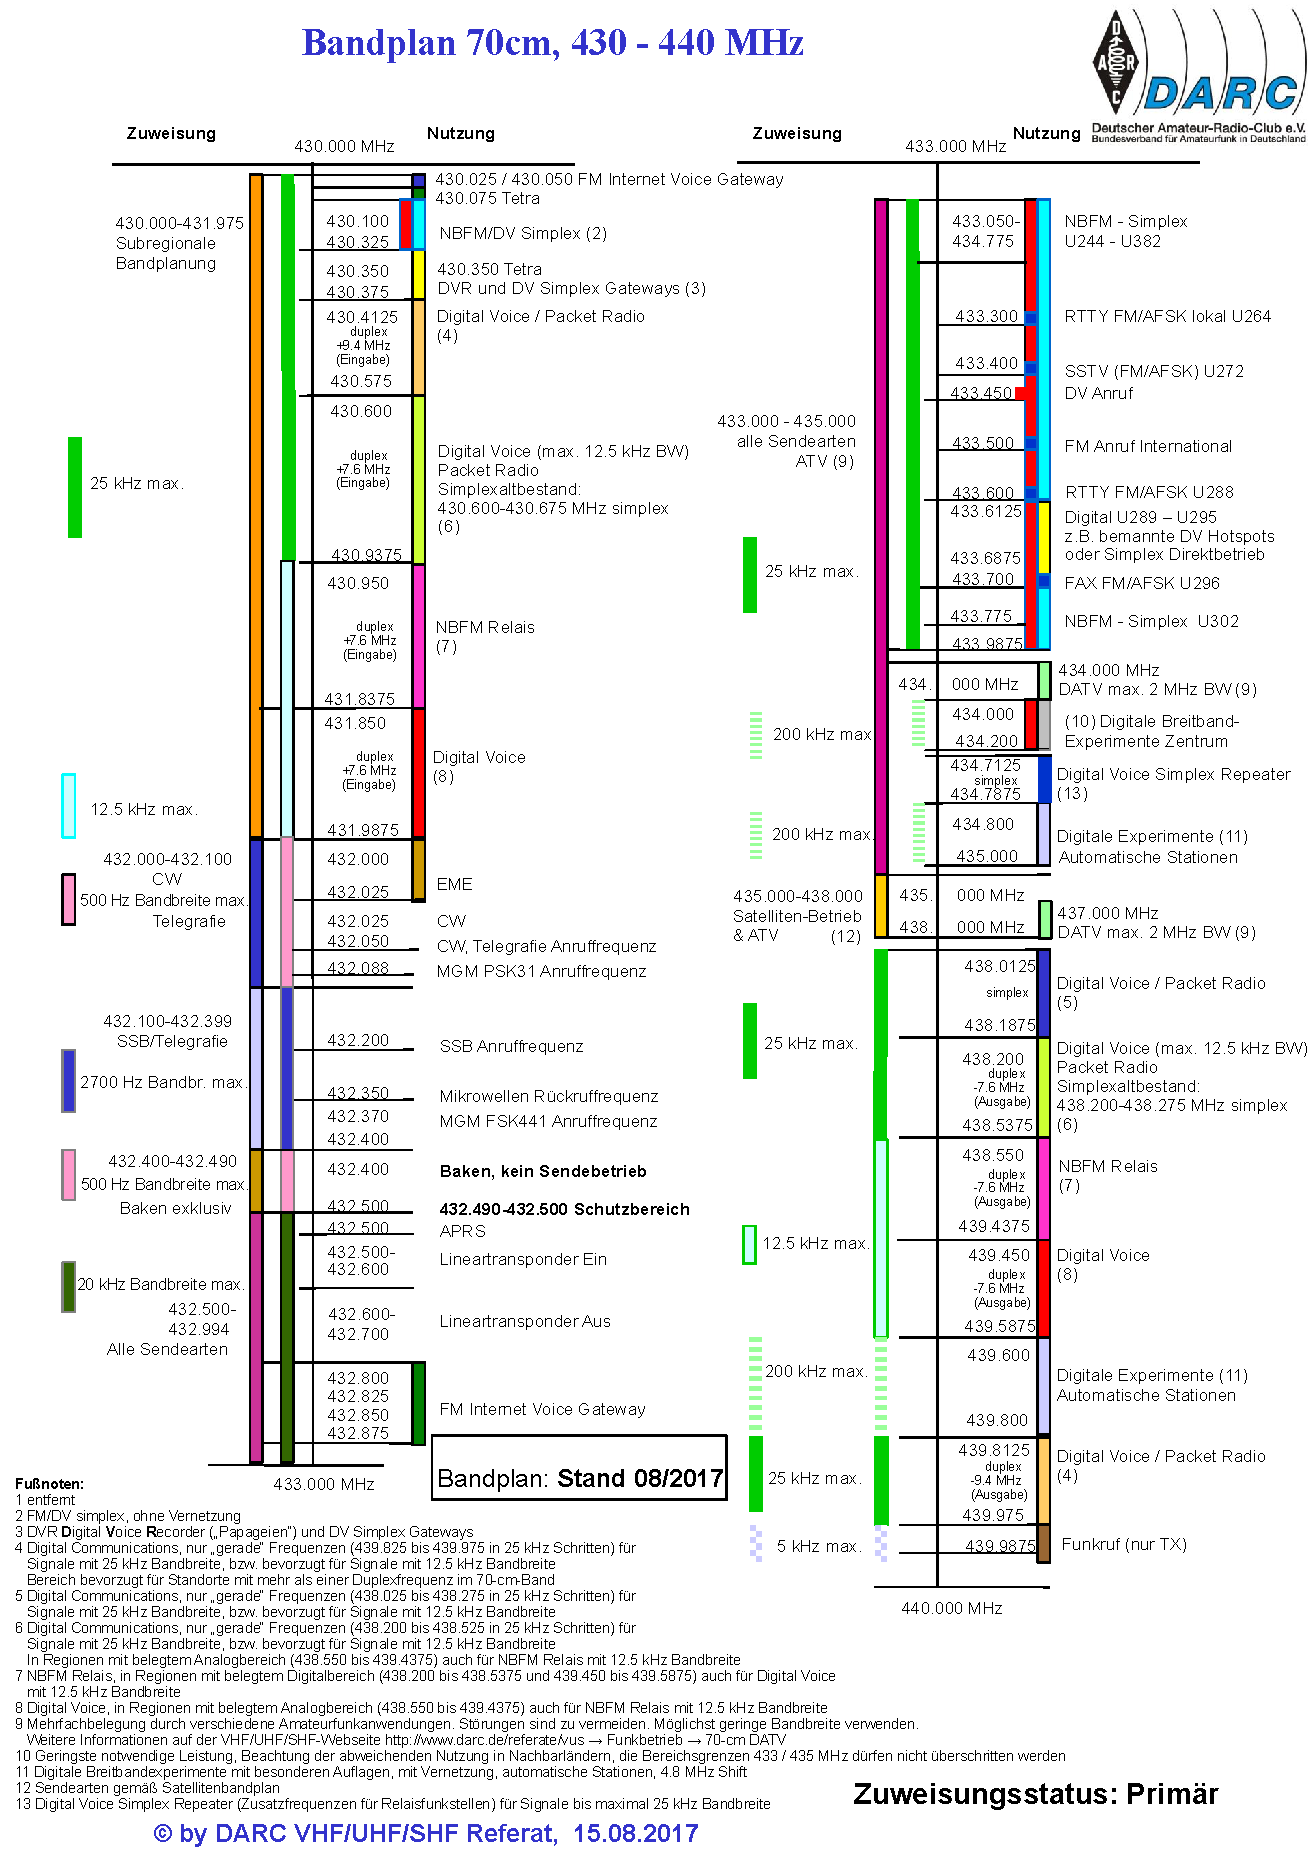
\includepdf[pages=-]{./bandplans/bandplan_70cm.pdf}

\fi 


\end{document}
